\section{Figures: Visual Object Models}
\label{app:vom-figures}

The diagrams below support Section~\ref{sec:visual-object-models}. They are
collected here so that the derivations in the main text are not interrupted by
full-page visuals; each is referenced from the relevant subsection.

\begin{figure}[ht]
  \centering
  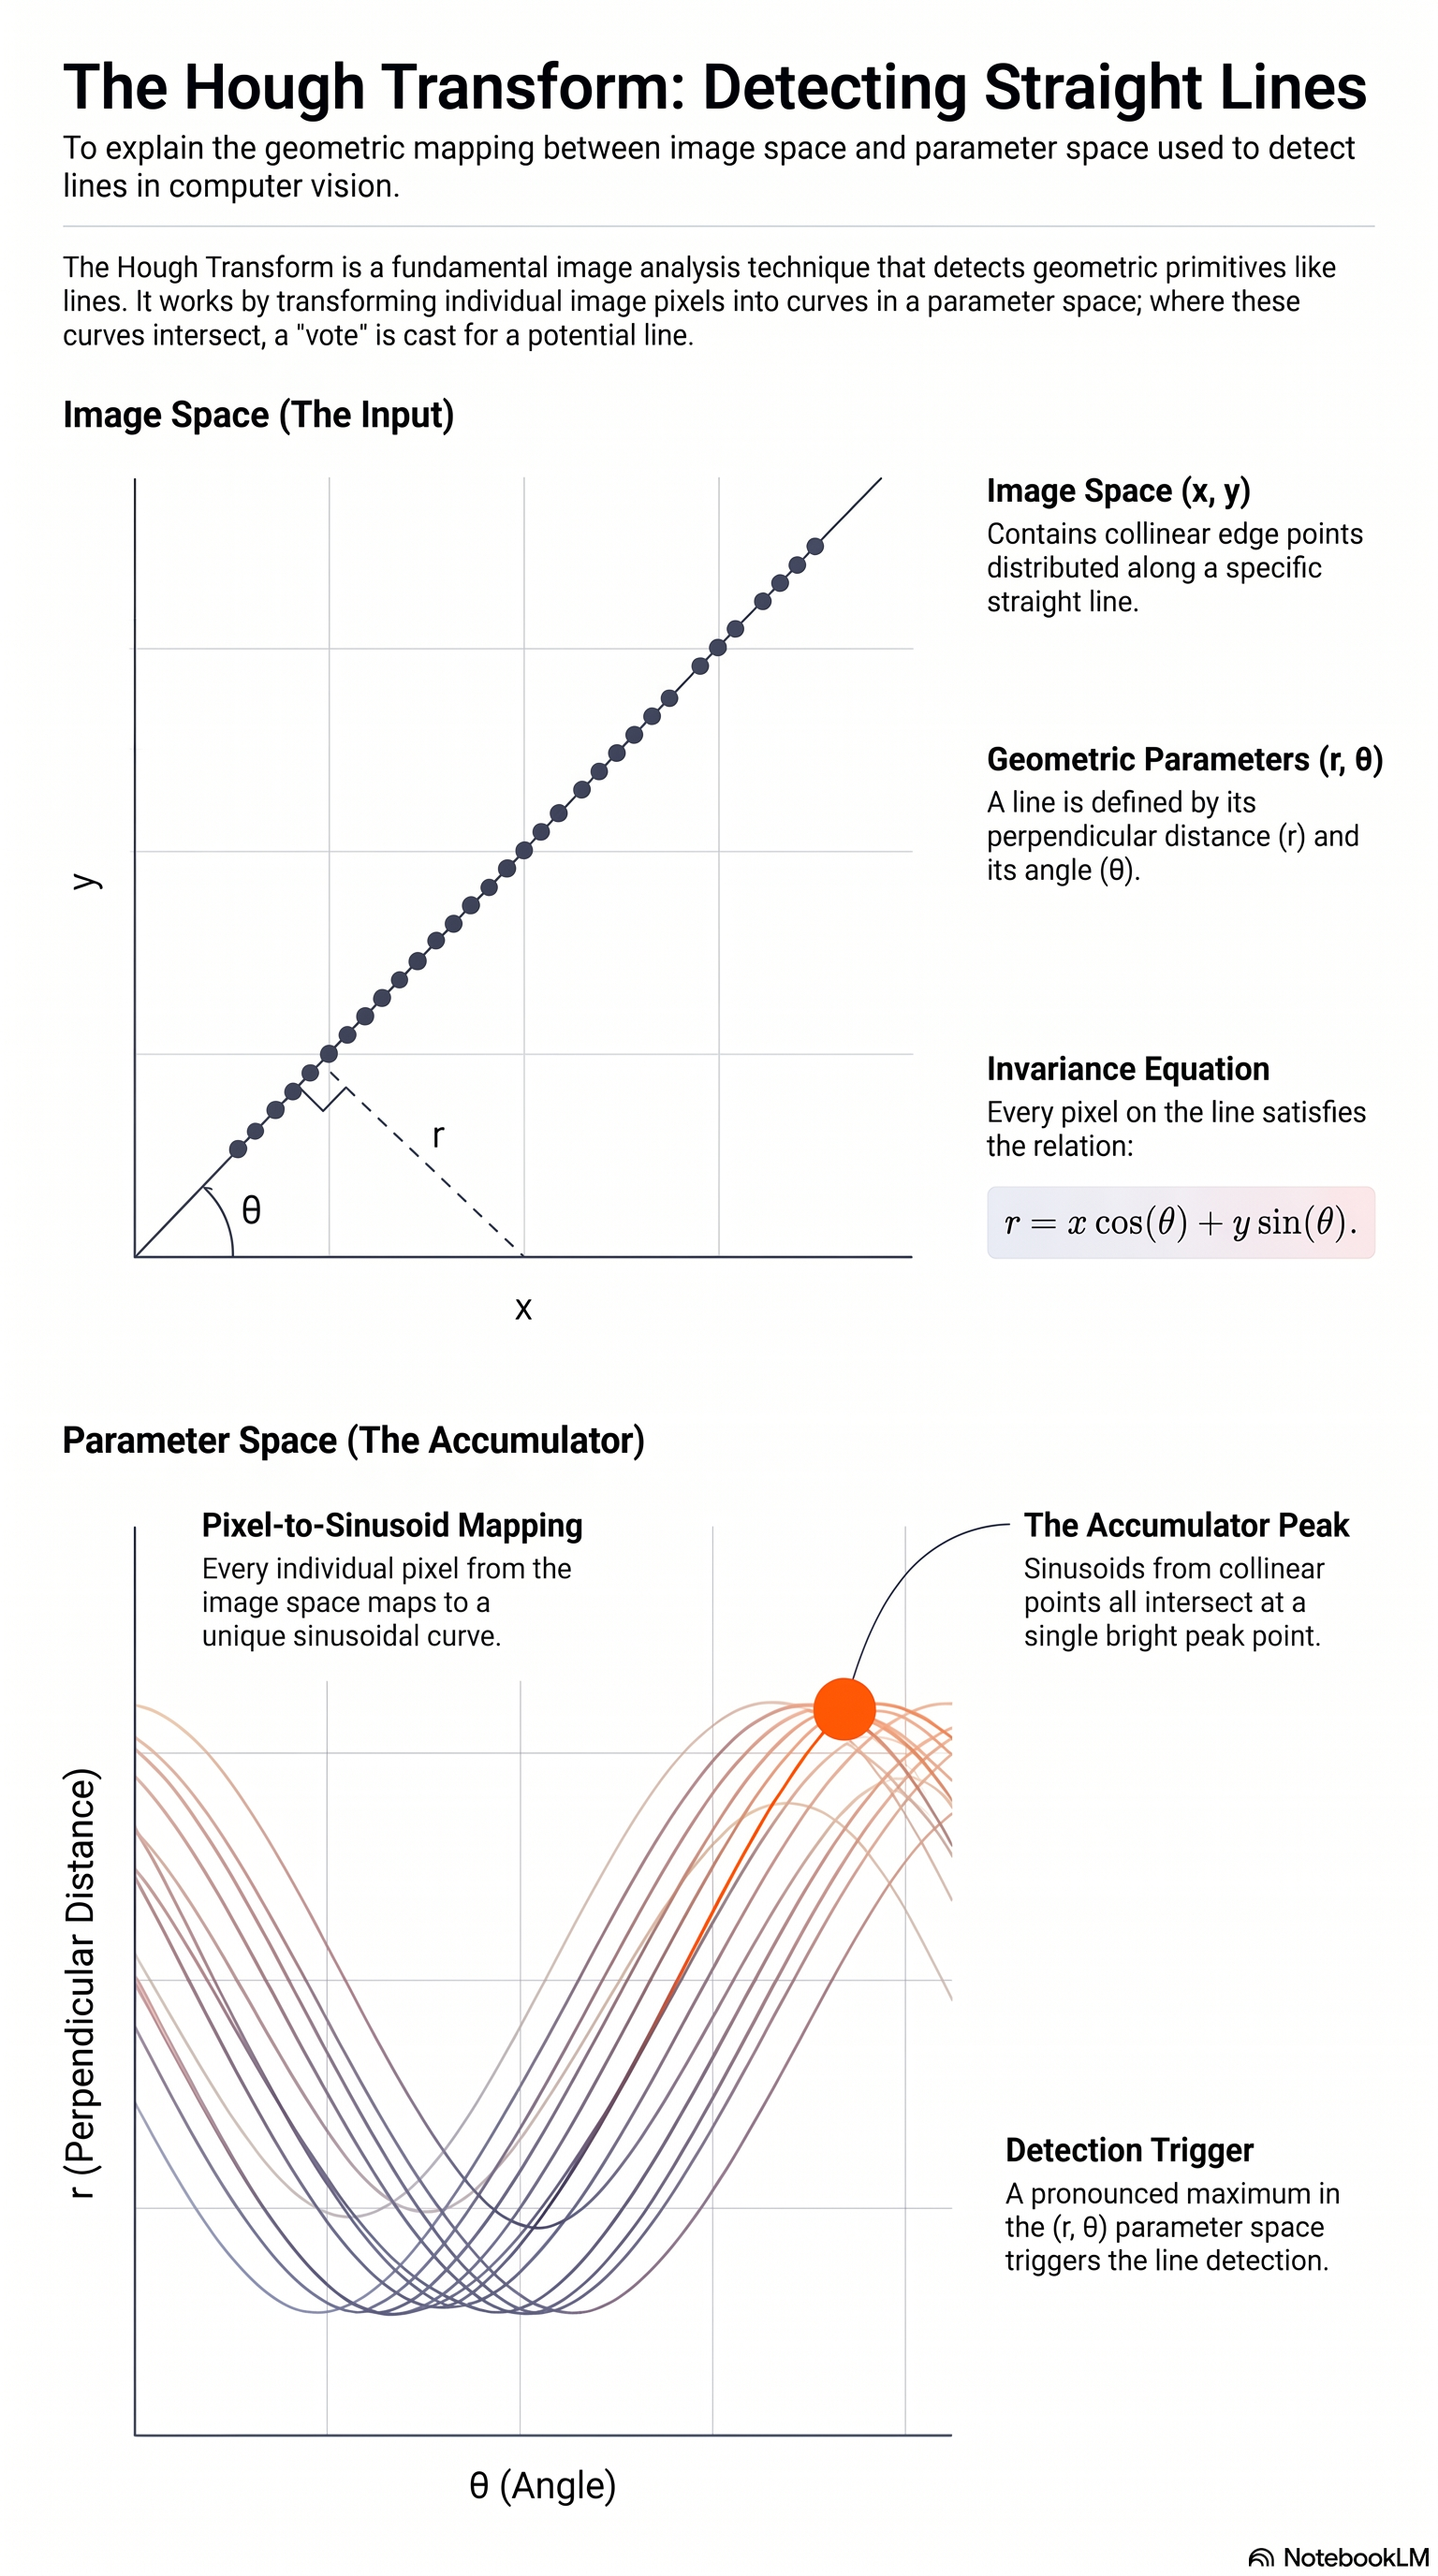
\includegraphics[width=0.66\textwidth]{figures/hough_duality_portrait.png}
  \caption{Hough duality for line detection. Collinear edge points in image
  space (top) all map to the same point in the $(r,\theta)$ accumulator
  (bottom); each individual point maps to a sinusoid, and the sinusoids intersect
  where the pixels agree. The pronounced peak triggers the detection.}
  \label{fig:hough-duality}
\end{figure}

\begin{figure}[ht]
  \centering
  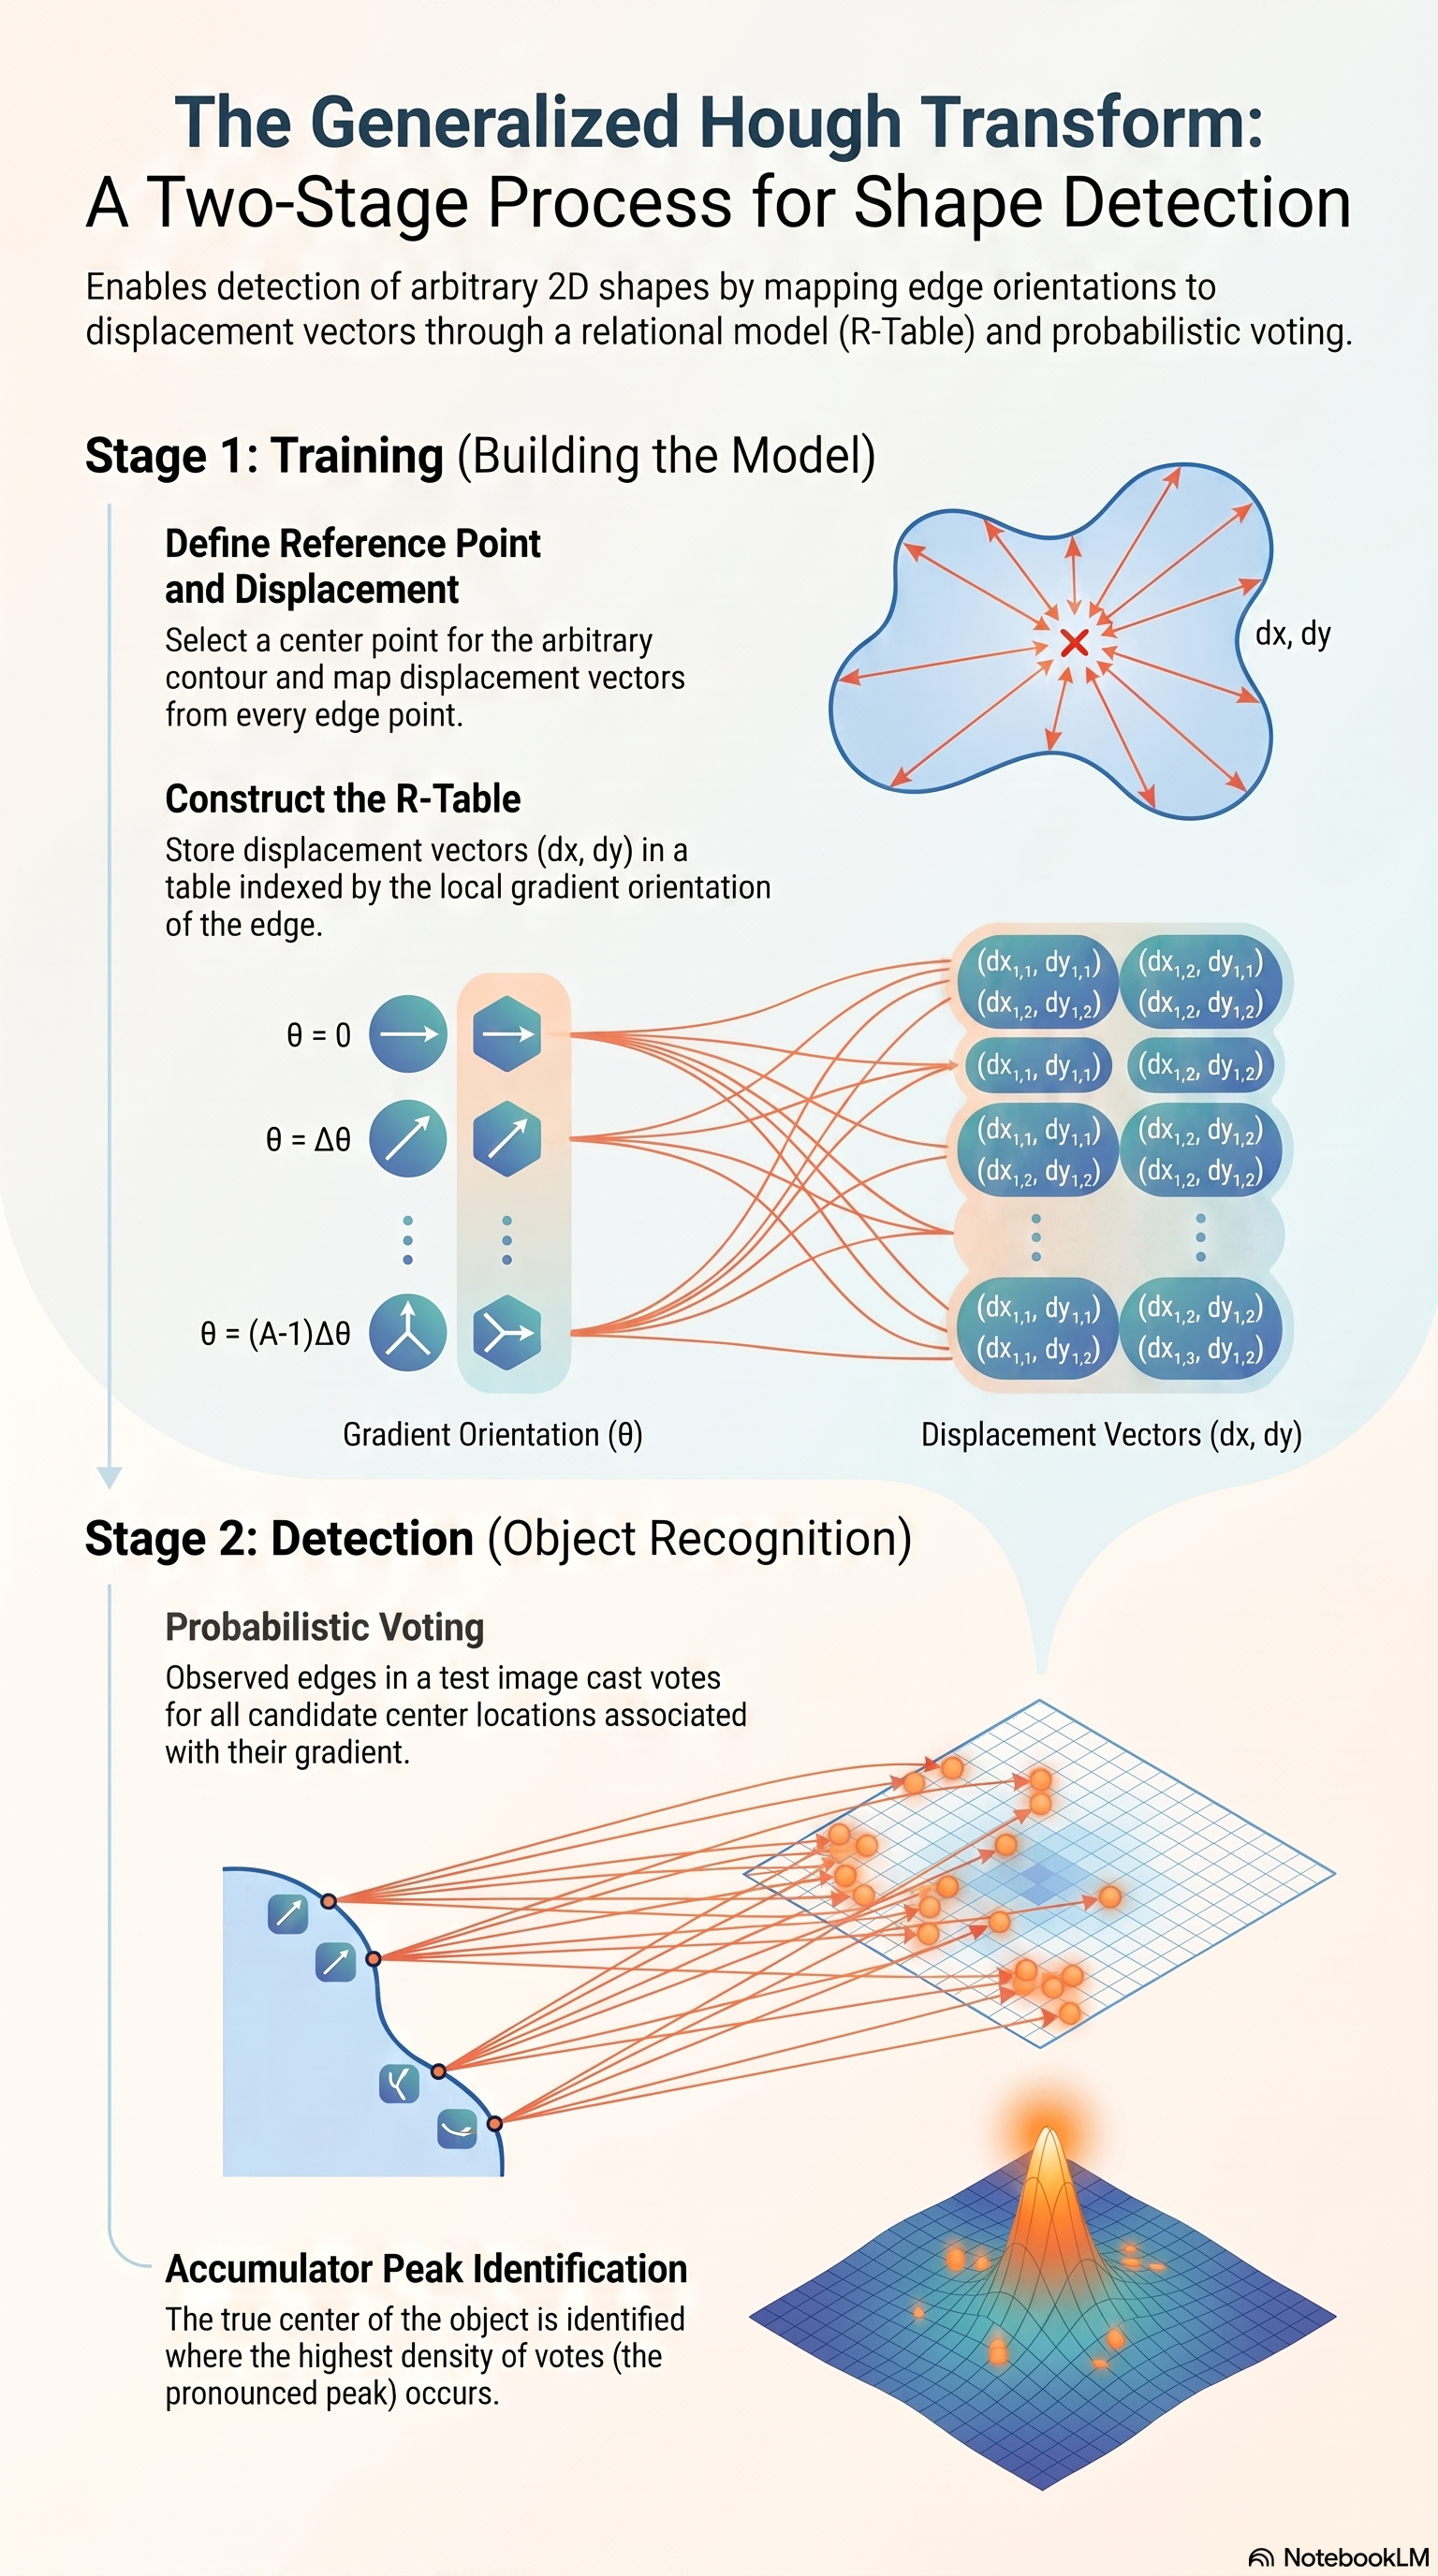
\includegraphics[width=0.66\textwidth]{figures/ght_rtable_portrait.png}
  \caption{Generalized Hough transform. Each model edge stores a displacement
  vector to the reference point, organized in the R-table by gradient
  orientation. Because the same orientation occurs at several places on the
  shape, one observed edge casts votes for several candidate centers; the true
  center is where votes accumulate.}
  \label{fig:ght-rtable}
\end{figure}

\begin{figure}[ht]
  \centering
  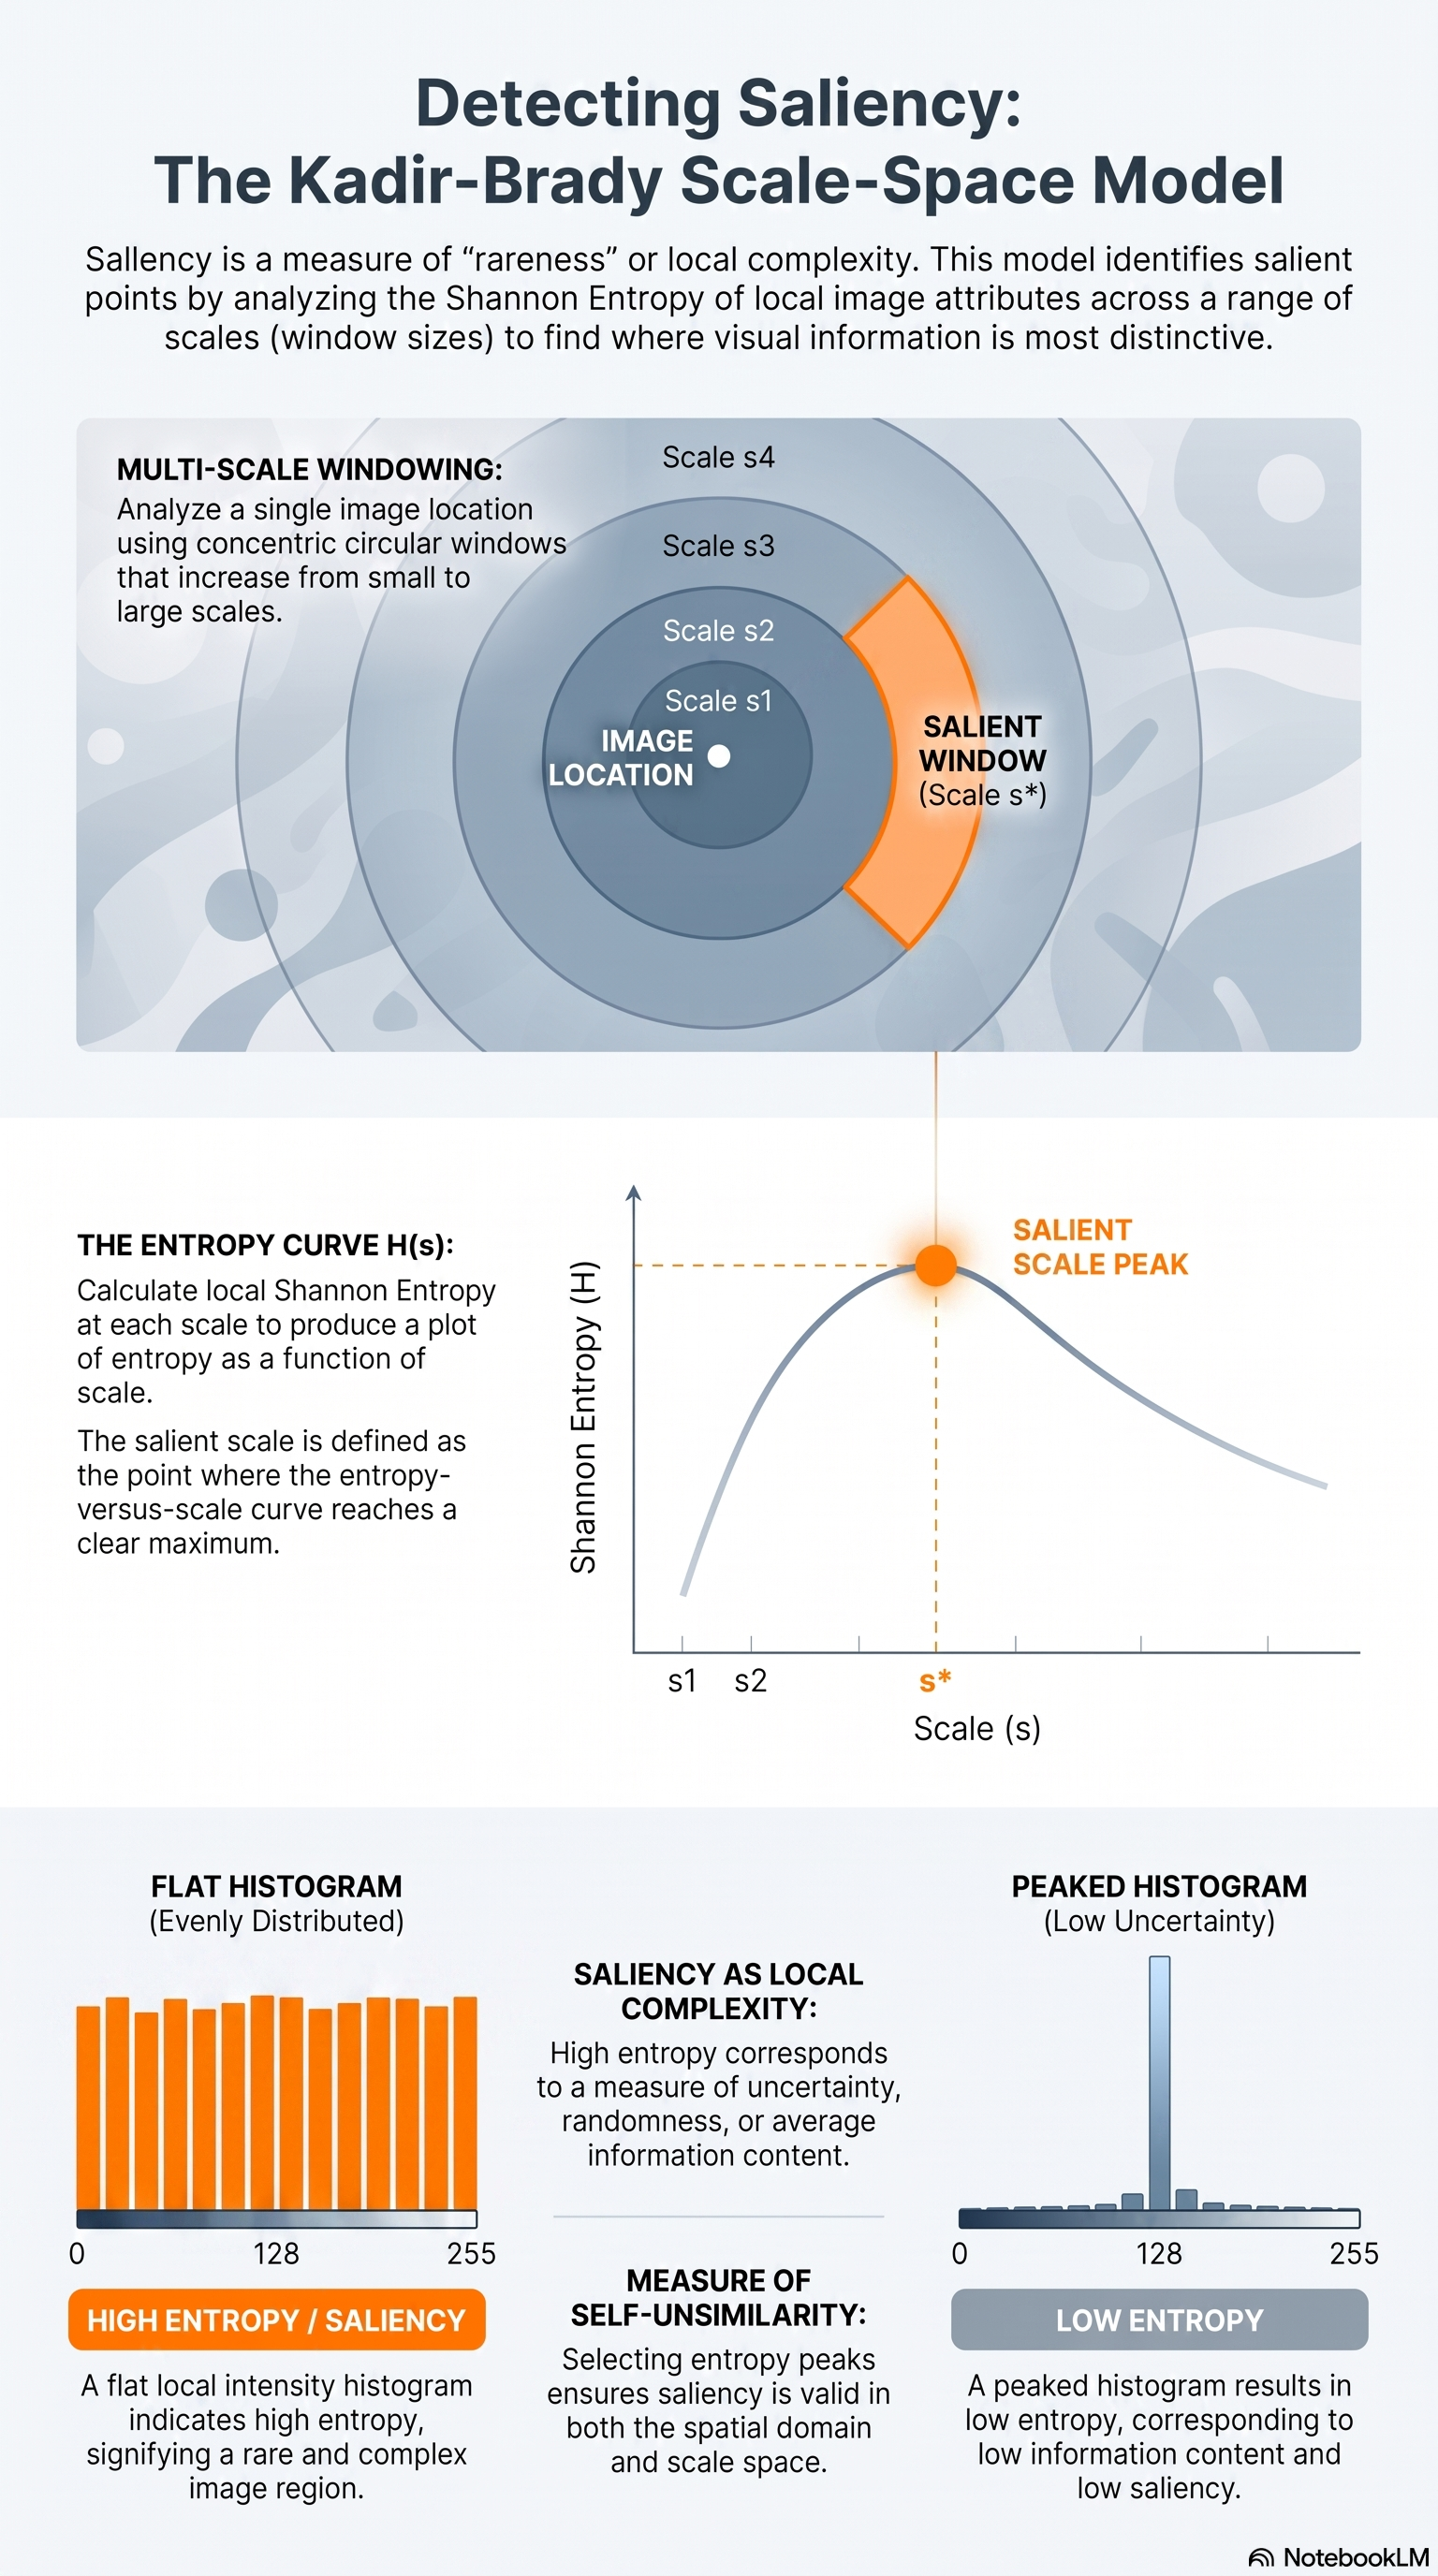
\includegraphics[width=0.66\textwidth]{figures/saliency_scale_portrait.png}
  \caption{Scale-space saliency. The same location is analyzed over a range of
  window sizes; entropy as a function of scale has a peak at the salient scale.
  A flat local histogram (high entropy) signals a rare, informative region,
  while the scale-localization weight discounts patches whose statistics barely
  change across scale.}
  \label{fig:saliency-scale}
\end{figure}

\begin{figure}[ht]
  \centering
  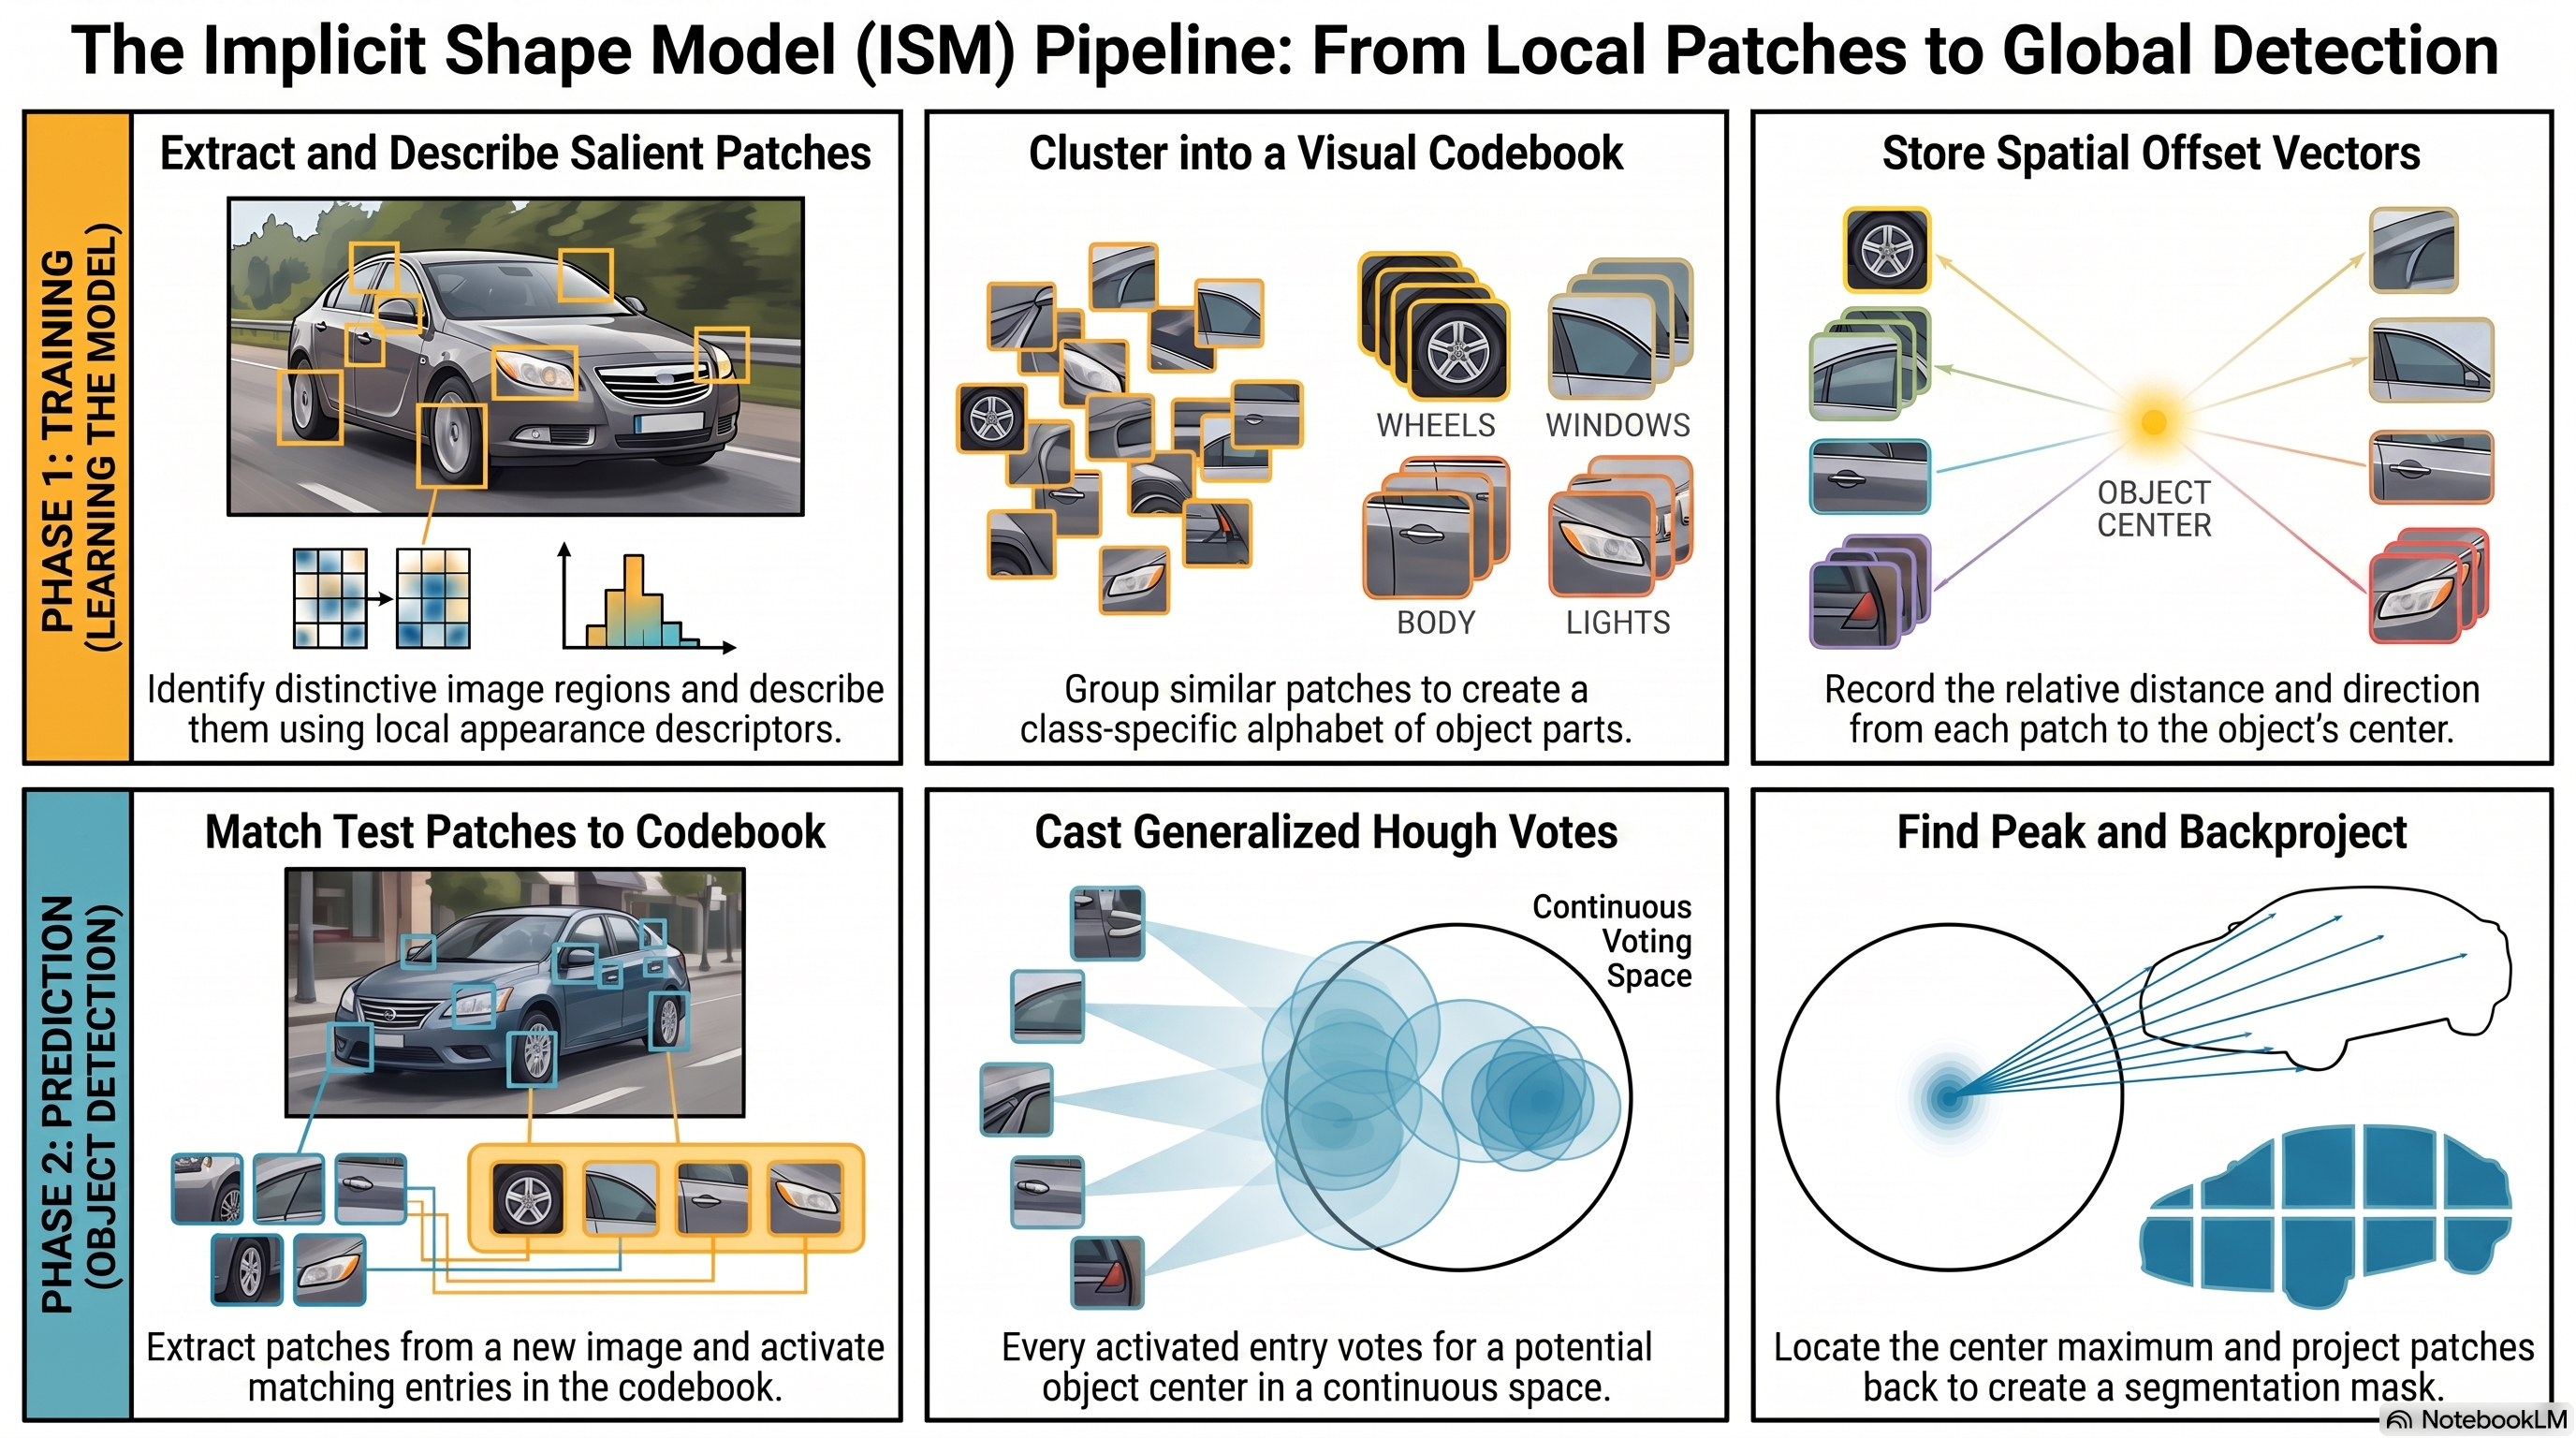
\includegraphics[width=\textwidth]{figures/ism_pipeline.png}
  \caption{The implicit shape model. Training (top row): salient patches are
  described, clustered into a codebook, and annotated with offset vectors to the
  object center. Prediction (bottom row): test patches are matched to the
  codebook, cast generalized Hough votes for the center, and the peak is
  back-projected to recover and segment the object.}
  \label{fig:ism-pipeline}
\end{figure}
